\section{Deferl\_bj78}
%

% - Purpose & Problem description:
%     These first two parts give reader short details about the test case,
%     the physical phenomena involved and specify how the numerical solution will be validated
%
\subsection{Purpose}
%
The aim of this case is to test the modelisation of depth-induced breaking. The
results are compared to laboratory data \cite{Battjes1978}
%
\subsection{Description of the problem}
%
Our test case corresponds to the ``run 15'' in Battles and Janssen
\cite{Battjes1978}. It is a rectilinear beach with a bar. The bathymetry of that
beach varies as shown on Figure \ref{bathybj}. The Battle and Janssen's
breaking model is used :

$ F_1=\int_{\theta=0}^{2\pi}F_0(\theta) d\theta$ where $F_0(\theta)$ is the
first moment of the action density spectrum over frequency.
$$
\frac{dF_1}{dt}=-\alpha_1Q_b\omega_1\frac{H_m^2}{8\pi}
$$
wherein $H_m$ denotes the maximum wave height. $Q_b$, the fraction of breaking
waves or breaking rate and $\alpha_1$ a numerical constant of order of 1.

$H_m$ is given by a relationship that is derived from de Miche's criterion:
$$
H_m=\frac{\gamma_1}{k_1}\tanh\left(\frac{\gamma_2k_1d}{\gamma_1} \right)
$$
wherein $k_1$ is related to $\omega_1$ by the dispersion relationship.

$Q_b$ is assessed, according to the Battjes and Janssen's theory as the
solution of the implicit equation:
$$
\frac{1-Q_b}{\ln Q_b}=-\frac{8F_1}{H_m^2}
$$
The ``directionnal'' version of that source term is based on the assumption
that the breaking does not change the directionnal distribution of energy. The
source term writes :
$$
Q_{br}(f,\theta)=- \frac{\alpha Q_bf_cH^2_m}{4}\frac{F(f,\theta)}{m_0}
$$
The values of numerical constants $\alpha_1$, $\gamma_1$ et $\gamma_2$ as
prescribed by Battjes and Janssen are 1, 0.88 and 0.8 respectively. These
values, however can and must be matched as a function of the camber of incident
waves and bottom slope. To that purpose the following keyword are provided :
{\it DEPTH-INDUCED BREAKING 1 (BJ) COEFFICIENT ALPHA} for $\alpha_1$, {\it
DEPTH-INDUCED BREAKING 1 (BJ) COEFFICIENT GAMMA1} for $\gamma_1$ and {\it
DEPTH-INDUCED BREAKING 1 (BJ) COEFFICIENT GAMMA2} for $\gamma_2$.

% - Reference:
%     This part gives the reference solution we are comparing to and
%     explicits the analytical solution when available;
%
%
%\subsection{Reference}
%

% - Physical parameters:
%     This part specifies the geometry, details all the physical parameters
%     used to describe both porous media (soil model in particularly) and
%     solute characteristics (dispersion/diffusion coefficients, soil <=> pollutant interactions...)
%
%
\subsection{Physical parameters}
%
The Battjes and Janssen's experiments were conducted in a channel and in
signle-direction wave conditions. We have then taken a little directionnal
spread(s=32) in order to set up similar condition.

% - Geometry and Mesh:
%     This part describes the mesh used in the computation
%
%
\subsection{Geometry and Mesh}
%
The domain is a 25~m by 12~m rectangle. The depth is constant over $y$ and
varrying with $x$ as shown on Figure \ref{bathybj}

\begin{figure} [!h]
\centering
\includegraphicsmaybe{[width=0.85\textwidth]}{../img/section1d.png}
%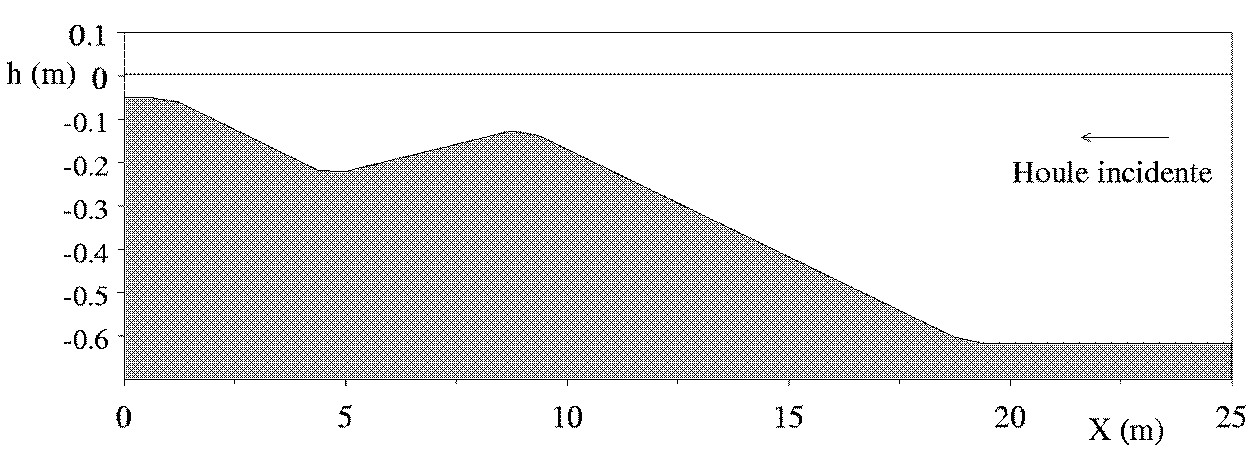
\includegraphics{bathy.png}
 \caption{section depth}
\label{bathybj}
\end{figure}

The mesh is free, it is made of 648 triangles and 373 points. The boundary has
96 points.
% - Initial and boundary conditions:
%     This part details both initial and boundary conditions used to simulate the case
%
%

\begin{figure} [!h]
\centering
\includegraphicsmaybe{[width=0.85\textwidth]}{../img/mesh.png}
%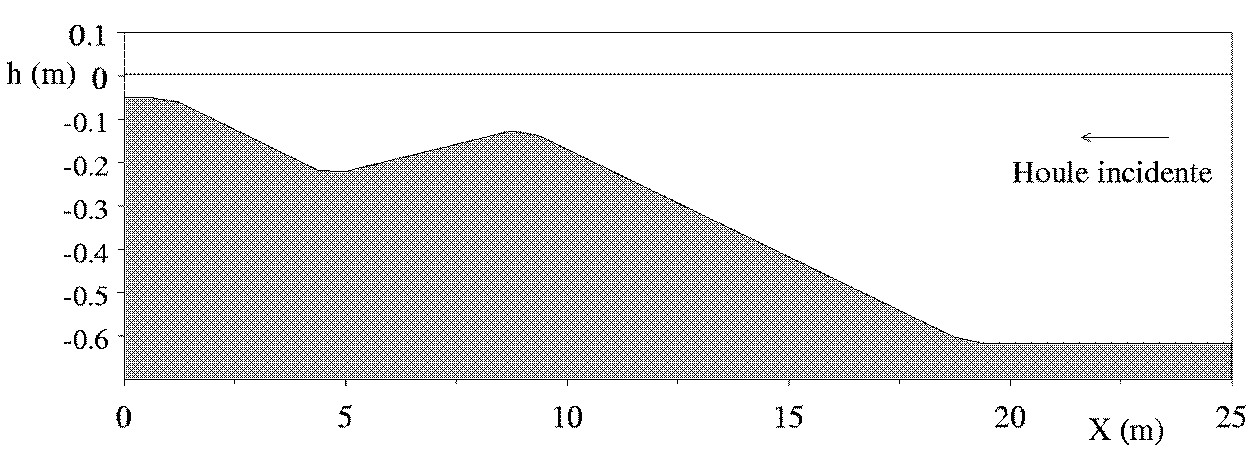
\includegraphics{bathy.png}
\caption{mesh of the domain.}
\label{meshbj}
\end{figure}
\subsection{Initial and Boundary Conditions}
The initial spectrum is null.

As for the boundary conditions, a Pierson-Moskowitz-typed spectrum is
prescribed at the west of the domain with a boundary peak frequency of 0.53Hz, a
significative heigth of 0.202~m and a boundary peak factor of 3.3. The boundary
principal direction is 270.
% - Numerical parameters:
%     This part is used to specify the numerical parameters used
%     (adaptive time step, mass-lumping when necessary...)
%
%
\subsection{Numerical parameters}
%
The time duration is 35~s with a time step of 0.35~s, the spectro-angular mesh
has 24 angles and 25 frequences spread on a geometric progression common ratio
1.1 with a minimum of 0.168874
% - Results:
%     We comment in this part the numerical results against the reference ones,
%     giving understanding keys and making assumptions when necessary.
%
%
\subsection{Results}
%
Figure \ref{resultbj1} displays the significant wave heights as computed by
Tomawac. One can see that Tomawac results are quite similar to the laboratory
data.

The effect of wave breaking on the mean frequency is not taken into account in
this case of Tomawac. As we suppose that energy dissipation does not affect the
spectro-angular energy spread. The energy transfers of the pre-breaking are
not taken into account.
\begin{figure} [!h]
\centering
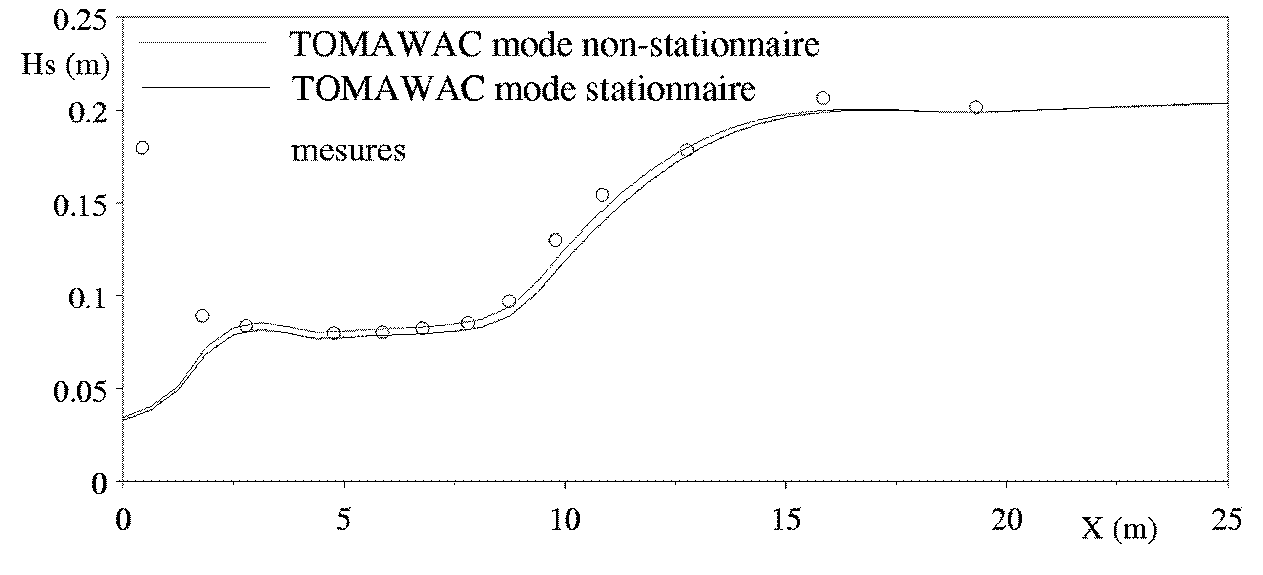
\includegraphics[width=0.5\textwidth]{results.png}
 \caption{comparison of the significative wave heigths}
\label{resultbj1}
\end{figure}
\begin{figure} [!h]
\centering
\includegraphicsmaybe{[width=0.75\textwidth]}{../img/results.png}
 \caption{Significative wave heigths for Battjes and Janssen Model}
\label{resultbj2}
\end{figure}
\begin{figure} [!h]
\centering
\includegraphicsmaybe{[width=0.75\textwidth]}{../img/results3.png}
 \caption{Significative wave heigths for Roelvink’s model}
\label{resultro3}
\end{figure}
\begin{figure} [!h]
\centering
\includegraphicsmaybe{[width=0.75\textwidth]}{../img/results4.png}
 \caption{Significative wave heigths for Izumiya and Horikawa’s turbulence model}
\label{resultih4}
\end{figure}
\subsection{Conclusion}
The breaking induced dissipation of energy is properly represented in Tomawac.
The effect on the mean frequency can be neglected.



